\chapter{Analyse, fortolkning og resultater}
\label{Ch:4}

I det følgende afsnit betragtes den empiri som er indsamlet i forbindelse med dette projekt.  I afsnit \vref{sec:4.1} betragtes den empiri som er indsamlet gennem det første spørgeskema, i afsnit \vref{sec:4.2} gennemgåes den indsamlede empiri fra spørgeskema to, og kapitlet afsluttes med et afsnit \vref{sec:4.3} hvor forskellige elevers skriftlige arbejde analyseres vha. TAP modellen.

\section{Spørgeskemaet}
\label{sec:4.1}
Som empirisk grundlag for dette projekt er der indsamlet data fra to spørgeskemaer samt fra elev afleveringer.  Besvarelserne, fra 1.g elever på Viborg Katedralskole, på spørgeskemaerne er indsamlet med Survey-Xact, der har været 117 besvarelser ud af 349 mulige besvarelser hvilket giver spørgeskemaet en svarprocent på \mbox{33,5 \%}. Undersøgelsen er blevet gennemført i forbindelse med praktisk eksperimentelt arbejde.  I forbindelse med det praktiske arbejde var der forbundet med et efterfølgende skriftligt arbejde. Spørgeskemaet blev gennemført i klasserne umiddelbart efter det praktiske arbejde og forud for det skriftlige arbejde blev påbegyndt. De 117 svar fordeler sig som vist på figur \vref{fig:4.1.a}. 

\begin{figure}[h!]
	\centering
	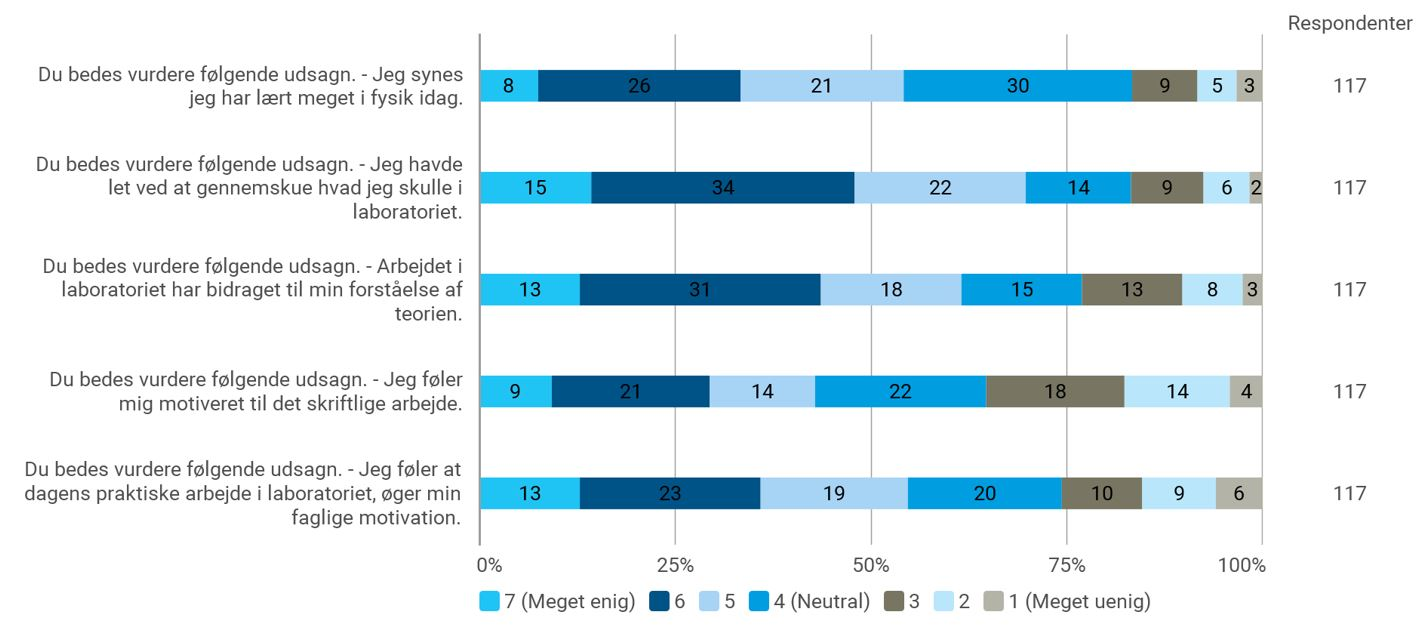
\includegraphics[width=0.9\textwidth]{Figs/Sammenlign}
	\caption{Det samlede datasæt for de fem spørgsmål med hver 117 respondenter fra en 1.g årgang på Viborg Katedralskole. Svar procenten for undersøgelsen er på omkring 33 \%. }
	\label{fig:4.1.a}
\end{figure}
Betragter man antallet af positive svar på de fem udsagn, hvor et svar regnes som positivt hvis der er svaret fire eller højere. Så vil gennemsnitet af besvarelserne være 66,32 \% af de afgivne svar i alle fem spørgsmål.  Hertil kunne det anfægtes om eleverne faktisk har forstået hvad de har svaret på, men her må man vise tilbage til Cronbach's $\alpha$ værdien som er blevet bestemt til 0.91 jf. afsnit \vref{sec:3.4}, denne værdi indikere at der er konsistens internt i undersøgelsen og at elevernes svar dermed har en hvis grad af konsistens. Generlt kan det uddrages ud af figur \vref{fig:4.1.a} at eleverne har let ved at gennemskue hvad de skulle i laboratoriet. Ligesom eleverne også mener at arbejdet i laboratoriet bar bidraget til deres forståelse af teorien. Ligeledes vurderer eleverne også at det praktiske arbejde i laboratoriet øver deres faglige motivation. Dog er eleverne mere tilbageholdende med at føle sig motiverede til det skriftlige arbejde. 


\section{Spørgeskema to}
\label{sec:4.2}

\section{Afleveringer}
\label{sec:4.3}
%\begin{figure}[h!]
%	\centering
%	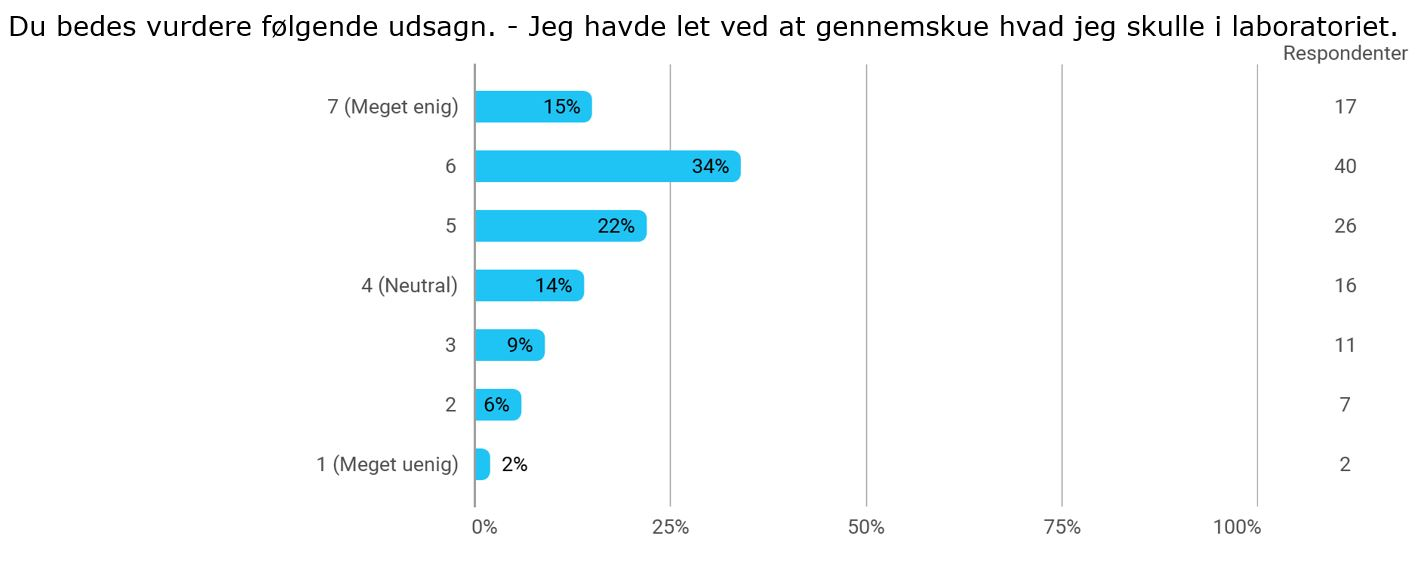
\includegraphics[width=0.9\textwidth]{Figs/Sp2}
%	\caption{Spørgeskema svar fra spørgsmål 2}
%	\label{fig:4.1.c}
%\end{figure}
%
%\begin{figure}[h!]
%	\centering
%	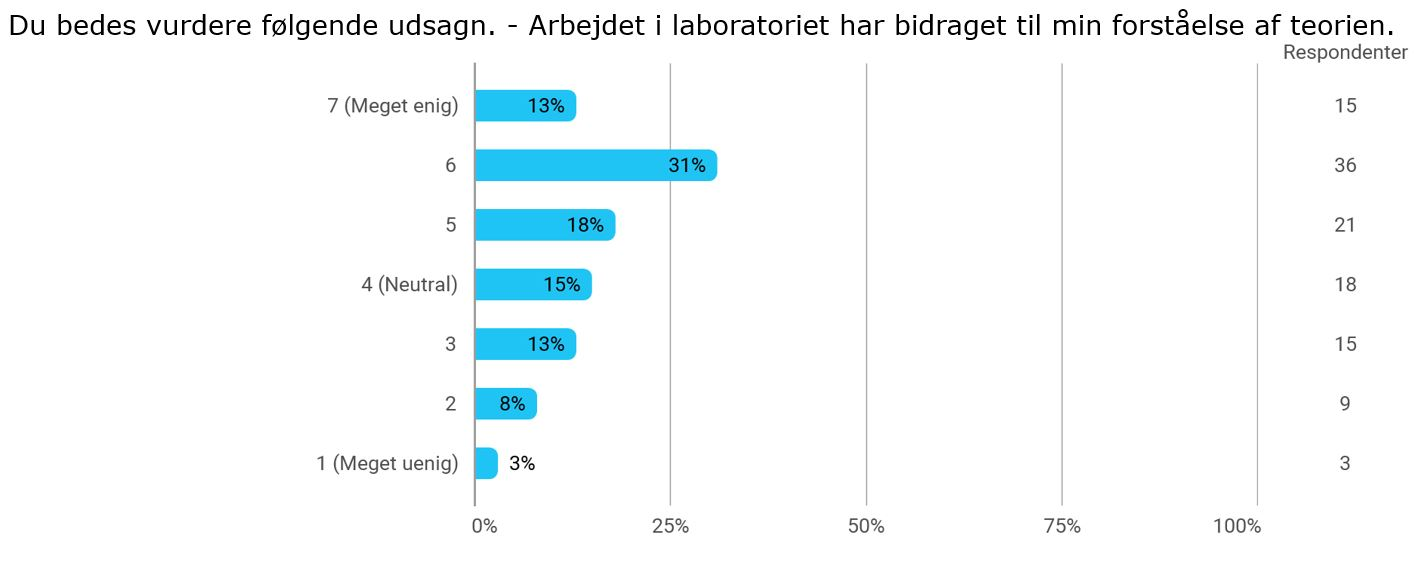
\includegraphics[width=0.9\textwidth]{Figs/Sp3}
%	\caption{Spørgeskema svar fra spørgsmål 3}
%	\label{fig:4.1.d}
%\end{figure}
%
%\begin{figure}[h!]
%	\centering
%	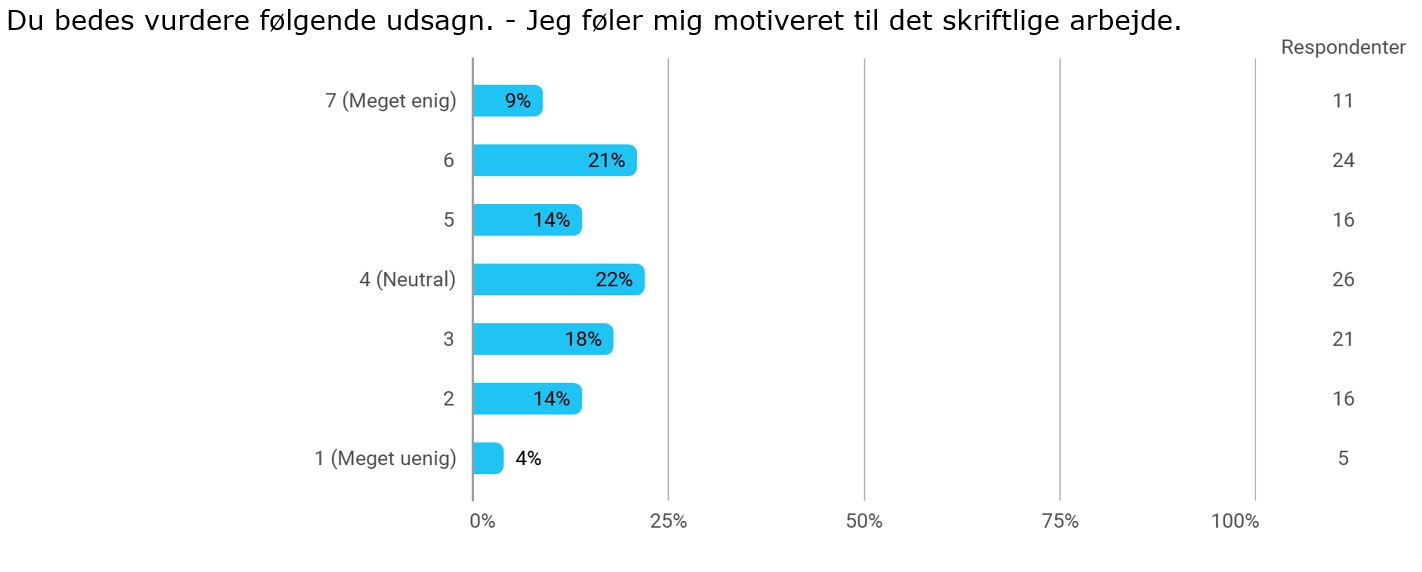
\includegraphics[width=0.9\textwidth]{Figs/Sp4}
%	\caption{Spørgeskema svar fra spørgsmål 4}
%	\label{fig:4.1.e}
%\end{figure}
%
%\begin{figure}[h!]
%	\centering
%	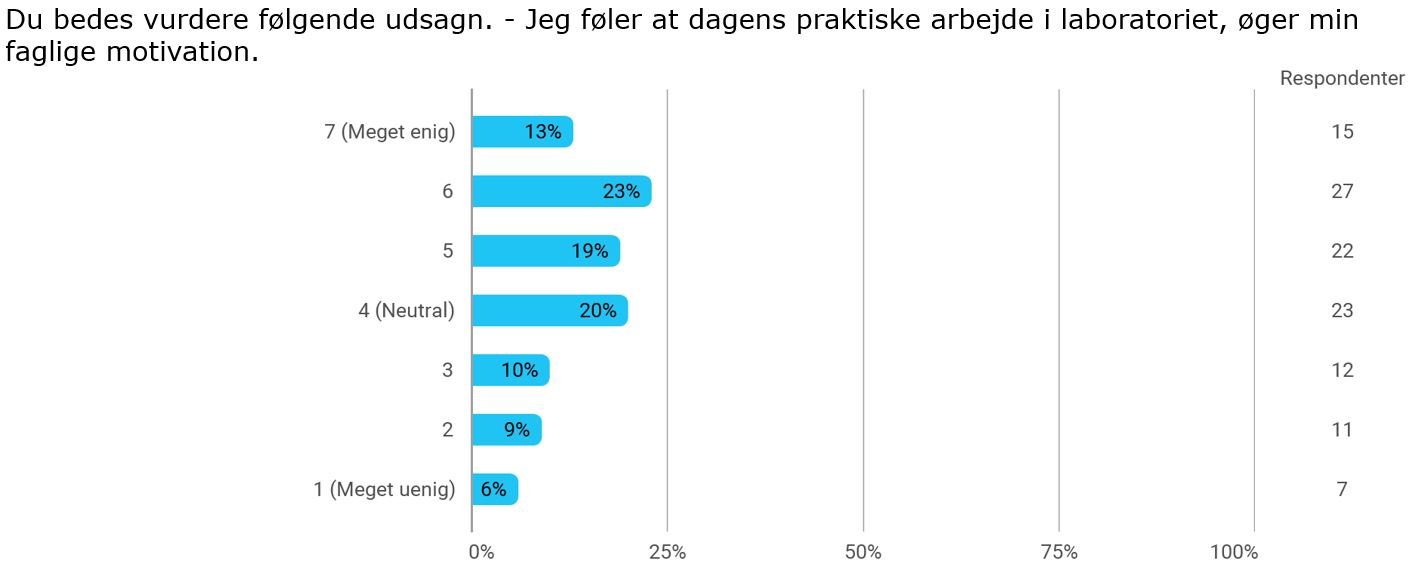
\includegraphics[width=0.9\textwidth]{Figs/Sp5}
%	\caption{Spørgeskema svar fra spørgsmål 5}
%	\label{fig:4.1.f}
%\end{figure}
